\section{Đặt vấn đề}
\label{section:1.1}

Trong những năm gần đây, xu hướng phát triển ứng dụng đa nền tảng ngày càng phổ biến do nhu cầu triển khai đồng thời trên nhiều hệ điều hành khác nhau như Android, iOS, Windows và Web. Thay vì xây dựng từng ứng dụng riêng biệt cho từng nền tảng, các doanh nghiệp và nhà phát triển mong muốn có thể tiết kiệm thời gian, chi phí và nguồn lực bằng cách xây dựng một ứng dụng duy nhất có khả năng hoạt động tốt trên nhiều thiết bị. 

\begin{figure}[H]
    \centering
    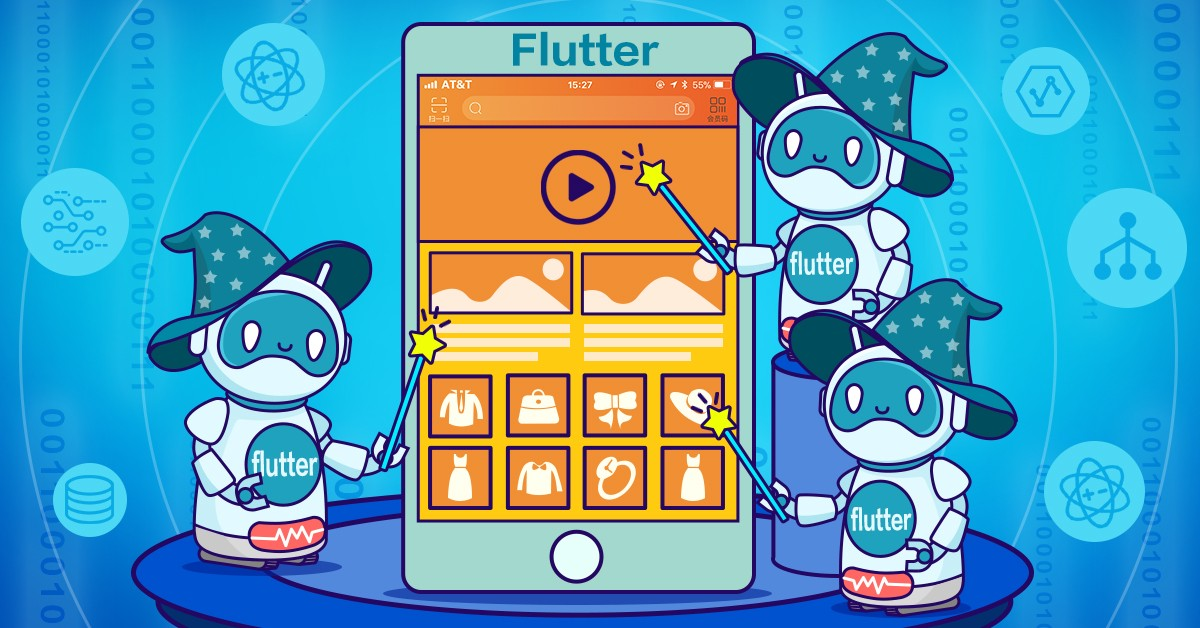
\includegraphics[width=0.8\textwidth]{Hinhve/Chuong1/flutter_image.jpeg}
    \caption{Framework Flutter}
    \label{fig:flutterimageintro}
\end{figure}

Flutter – một framework được phát triển bởi Google – cùng với ngôn ngữ Dart, đã trở thành một trong những lựa chọn hàng đầu cho phát triển ứng dụng đa nền tảng. Với khả năng hỗ trợ giao diện người dùng phong phú, hiệu suất cao và công nghệ “hot reload”, Flutter đã nhanh chóng chiếm lĩnh thị trường và được cộng đồng phát triển ứng dụng đón nhận rộng rãi.

<<<<<<< HEAD
Trong bối cảnh đó, việc nghiên cứu và nắm bắt tổng quan về Dart và Flutter không chỉ mang lại lợi ích học thuật cho sinh viên ngành công nghệ thông tin, mà còn mở ra những cơ hội nghề nghiệp tiềm năng trong thị trường lao động hiện nay. Chính vì vậy, đề tài này được thực hiện nhằm mục tiêu tìm hiểu, phân tích và hệ thống hóa kiến thức cơ bản về Dart và Flutter – từ cú pháp, lập trình hướng đối tượng trong Dart, đến kiến trúc Flutter và cách xây dựng một ứng dụng cơ bản.
=======
Trong bối cảnh đó, việc nghiên cứu và nắm bắt tổng quan về Dart và Flutter không chỉ mang lại lợi ích học thuật cho sinh viên ngành công nghệ thông tin, mà còn mở ra những cơ hội nghề nghiệp tiềm năng trong thị trường lao động hiện nay. Đề tài này nhằm mục tiêu tìm hiểu, phân tích và hệ thống hóa kiến thức cơ bản về Dart và Flutter – từ cú pháp, lập trình hướng đối tượng trong Dart, đến kiến trúc Flutter và cách xây dựng một ứng dụng cơ bản.
>>>>>>> e99cf771c83e18ae8ecc6bb8d6dc5eff79ee4fb1

\section{Mục tiêu và phạm vi đề tài}
\label{section:1.2}

Hiện nay, nhiều công nghệ như React Native, Xamarin hay NativeScript đã được phát triển nhằm hỗ trợ xây dựng ứng dụng đa nền tảng. Tuy nhiên, các framework này vẫn tồn tại nhiều hạn chế về hiệu suất, khả năng tùy biến giao diện, và độ tương thích với hệ điều hành. Flutter nổi lên như một giải pháp khắc phục nhiều nhược điểm trên nhờ kiến trúc widget thống nhất, khả năng kết xuất (rendering) mạnh mẽ, và hiệu năng tiệm cận native.

Mặc dù cộng đồng phát triển Flutter đang phát triển nhanh chóng, sinh viên vẫn gặp khó khăn trong việc tiếp cận kiến thức một cách hệ thống do thiếu tài liệu tổng hợp rõ ràng, dễ hiểu. Do đó, đề tài này hướng đến việc biên soạn và trình bày tổng quan một cách logic, trực quan và đầy đủ nhất có thể về Dart và Flutter, phục vụ mục đích học tập, giảng dạy và phát triển ứng dụng thực tế.

<<<<<<< HEAD
Phạm vi đề tài tập trung vào các nội dung cơ bản về Dart (bao gồm lịch sử của ngôn ngữ, cú pháp, lập trình hướng đối tượng, hàm, quản lý gói, ...) và Flutter (kiến trúc, widget, quản lý trạng thái, xây dựng ứng dụng cơ bản). Nhóm định hướng đề tài theo phương pháp nghiên cứu tổng hợp tài liệu kết hợp thực nghiệm cài đặt. Các nội dung sẽ được hệ thống hóa lại thành các chủ đề logic: từ giới thiệu ngôn ngữ Dart, các cú pháp cơ bản của ngôn ngữ Dart, lập trình hướng đối tượng, cấu trúc ứng dụng Flutter, đến cách tạo ứng dụng đầu tiên với quản lý trạng thái đơn giản.
=======
Phạm vi đề tài tập trung vào các nội dung cơ bản về Dart (bao gồm lịch sử của ngôn ngữ, cú pháp, lập trình hướng đối tượng, hàm, quản lý gói, v.v.) và Flutter (kiến trúc, widget, quản lý trạng thái, xây dựng ứng dụng cơ bản). Nhóm định hướng đề tài theo phương pháp nghiên cứu tổng hợp tài liệu kết hợp thực nghiệm cài đặt. Các nội dung sẽ được hệ thống hóa lại thành các chủ đề logic: từ giới thiệu ngôn ngữ Dart, các cú pháp cơ bản của ngôn ngữ Dart, lập trình hướng đối tượng, cấu trúc ứng dụng Flutter, đến cách tạo ứng dụng đầu tiên với quản lý trạng thái đơn giản.
>>>>>>> e99cf771c83e18ae8ecc6bb8d6dc5eff79ee4fb1

